\documentclass[xcolor=svgnames,9pt,english,aspectratio=169,t]{beamer}
%\documentclass[xcolor=svgnames,9pt,english,handout,aspectratio=169,t]{beamer}
\newcommand{\handout}{0}

% =====================================================================
% POLI 450A (2026) --- shared TEMPLATE layer.
%
% Input from each lecture near the top of its file, BEFORE
% ../course_theme.tex (metropolis must be selected before the course
% palette overrides it):
%
%   \documentclass[xcolor=svgnames,9pt,english,aspectratio=169]{beamer}
%   \newcommand{\handout}{0}
%   % =====================================================================
% POLI 450A (2026) --- shared TEMPLATE layer.
%
% Input from each lecture near the top of its file, BEFORE
% ../course_theme.tex (metropolis must be selected before the course
% palette overrides it):
%
%   \documentclass[xcolor=svgnames,9pt,english,aspectratio=169]{beamer}
%   \newcommand{\handout}{0}
%   % =====================================================================
% POLI 450A (2026) --- shared TEMPLATE layer.
%
% Input from each lecture near the top of its file, BEFORE
% ../course_theme.tex (metropolis must be selected before the course
% palette overrides it):
%
%   \documentclass[xcolor=svgnames,9pt,english,aspectratio=169]{beamer}
%   \newcommand{\handout}{0}
%   \input{../course_preamble.tex}
%   \input{../course_theme.tex}
%   \graphicspath{{./}{./figs/}}
%   \title[Short title]{450A Political Methodology I}
%   \subtitle{Lecture N: ...}
%
% Modeled on the 2026 Northwestern workshop template
% (Teaching/PanelData/_latex/2026/202608_Northwestern/workshop_preamble.tex).
%
% SCOPE: theme, beamer layout, packages, the roadmap hooks, and --- unlike
% the Northwestern decks --- the notation macros. The 450A lectures
% grew from one common ancestor, so their macro blocks agree wherever they
% overlap; merging them is safe. Three points where they had drifted are
% resolved here, and each is flagged inline below.
% =====================================================================

\usetheme{metropolis}
\metroset{sectionpage=none, subsectionpage=none, numbering=none}
\setbeamertemplate{navigation symbols}{}

\setbeamersize{text margin left=5mm, text margin right=5mm}
\setbeamertemplate{itemize/enumerate body begin}{\leftmargini=1.5em\relax}
\setbeamertemplate{itemize/enumerate subbody begin}{\leftmarginii=1.5em\relax}
\setbeamertemplate{itemize/enumerate subsubbody begin}{\leftmarginiii=1.5em\relax}

% ----------------------------------------------------------- top alignment
% Every deck passes the t class option, so beamer applies the frame key
% below to every frame (explicit [plain,c] frames — title page, roadmaps —
% stay centered). Beamer's stock t key puts a rigid .2cm pad above the
% content; frames sized to this template's full-height ceilings then run
% Overfull \vbox by up to that pad. Same key as beamerbaseframe.sty, with
% one change: the pad may shrink to zero when the frame is full.
\makeatletter
\define@key{beamerframe}{t}[true]{% top
  \beamer@frametopskip=.2cm plus .5\paperheight minus .2cm\relax%
  \beamer@framebottomskip=0pt plus 1fill\relax%
  \beamer@frametopskipautobreak=\beamer@frametopskip\relax%
  \beamer@framebottomskipautobreak=\beamer@framebottomskip\relax%
}

% ------------------------------------------------- slide-top check (2026-10-11)
% A slide whose content is too tall for the frame is squeezed: the pad above
% shrinks and its content starts higher than on other slides, so a figure
% "wobbles" when the class steps from one slide to the next (Lecture 4-1,
% slides 1-2, 2026-10-11). The marker below records where each slide's
% content starts (a whatsit: it adds no space and moves nothing).
% `python3 ../check_slides.py lec<N>` then lists every slide that starts
% higher than the deck's normal position. That list must be empty.
% Recorded per slide: page, frame number, content-top y (sp), the room left
% below the title bar, and P for a plain frame (title page, roadmaps).
\providecommand\slidetop[5]{}
\AtBeginDocument{\immediate\write\@auxout{\string\providecommand\string\slidetop[5]{}}}
\def\beamer@markframetop{%
  \pdfsavepos
  \edef\beamer@marktmp{\noexpand\write\noexpand\@auxout{\string\slidetop
    {\noexpand\thepage}{\noexpand\insertframenumber}{\noexpand\the\noexpand\pdflastypos}%
    {\number\beamer@frametextheight}{\ifbeamer@plainframe P\else N\fi}}}%
  \beamer@marktmp}
\RequirePackage{etoolbox}
\patchcmd{\endbeamer@frameslide}
  {\vskip\beamer@frametopskip}
  {\vskip\beamer@frametopskip\beamer@markframetop}
  {}{\PackageWarning{course_preamble}{slide-top marker not installed}}
\makeatother

% ---------------------------------------------------------------- packages
\usepackage{xcolor}
\usepackage{colortbl}
\usepackage{amsmath}
\usepackage{amsfonts}
\usepackage{amssymb}
\usepackage{bm}
\usepackage{graphicx}
\usepackage{multirow}
\usepackage{fancyvrb}
\usepackage{listings}
\usepackage{tikz}
\usetikzlibrary{arrows.meta,positioning,decorations.pathreplacing}

% --------------------------------------------------------- figure fitting
% Default bounding box for every \includegraphics that does not override it.
% With keepaspectratio the image is scaled to fit *inside* width x height, so
% a figure can never run past the side margins or off the bottom of a slide.
% Options given at the call site override these on a per-key basis: e.g.
% [width=.6\linewidth] narrows the box but keeps the height ceiling.
% \figmaxheight is set at \begin{document}: beamer only computes the final
% \textheight once the head/foot templates are known. 0.80 is just under what a
% frame with a title and one line of text can hold (measured: 0.834\textheight);
% a frame that needs more room for text can lower it locally.
\newlength{\figmaxheight}
\AtBeginDocument{\setlength{\figmaxheight}{0.80\textheight}}
\setkeys{Gin}{width=\linewidth,height=\figmaxheight,keepaspectratio}

% -------------------------------------------------------- roadmap frames
% Identical in all lectures. A lecture that does not want the
% subsection roadmap clears it after the \input with \AtBeginSubsection[]{}.
% hideothersubsections is load-bearing, not cosmetic: lecture 4 had 13
% subsections before it was split into 4-1, 4-2 and 4-3 (2026-10-09), and a
% full contents list ran off the top and bottom of the slide. Hiding the other sections' subsections caps the list at 10 lines.
\subject{Talks}
% No back-to-back roadmaps (Yiqing, 2026-10-11): when a subsection starts right
% after its section's roadmap, with no content slide in between, its own
% roadmap would repeat the one just shown (5-1's handout showed "Two Cases"
% twice), so it is skipped. The section roadmap records the frame count; the
% subsection roadmap appears only if a content slide has come since.
\makeatletter
\def\course@secframe{-1}
\AtBeginSection[]
{
  \begin{frame}[plain,c]
    \frametitle{}
    \tableofcontents[currentsection,hideothersubsections]
    \addtocounter{framenumber}{-1}
  \end{frame}
  \xdef\course@secframe{\the\c@framenumber}
}
\AtBeginSubsection[]
{
  \ifnum\c@framenumber=\course@secframe\relax\else
  \begin{frame}[plain,c]
    \frametitle{}
    \tableofcontents[currentsection,currentsubsection,hideothersubsections]
    \addtocounter{framenumber}{-1}
  \end{frame}
  \fi
}
\makeatother

% ------------------------------------------------------ theorem environments
\newtheorem{assumption}{Assumption}
\newtheorem{iass}{Identification Assumption}
\newtheorem{ires}{Identification Result}
\newtheorem{estm}{Estimand}
\newtheorem{esti}{Estimator}
\newtheorem{question}{Question}
\newtheorem{answer}{Answer}
\newtheorem{proposition}{Proposition}

% =====================================================================
% Notation
% =====================================================================
\definecolor{dgreen}{rgb}{0,.6,0.8}

\renewcommand\r{\right}
\renewcommand\l{\left}
\newcommand{\bs}{\boldsymbol}
\newcommand{\mb}{\mathbf}
\newcommand{\real}{\mathbb{R}}
\newcommand{\cN}{\mathcal{N}}
\newcommand{\E}{\mathbb{E}}
\newcommand{\V}{\mathbb{V}}

% MERGE NOTE 1. Lecture 2-4 set \epsilon to \varepsilon; the other twelve
% left it at the upright default. Adopting \varepsilon course-wide so the
% error term looks the same in every lecture.
\renewcommand{\epsilon}{\varepsilon}

% MERGE NOTE 2. Lecture 2-4 wrote its vectors as \bm (bold italic); the other
% twelve use \mathbf (bold upright). \mathbf wins --- it is the convention in
% eleven of the thirteen decks and in the course's matrix lectures. Only
% \iid, \E, \cN and \Var from that block are actually used in 2-4's body.
\renewcommand{\u}{\ensuremath{\mb{u}}}
\renewcommand{\v}{\ensuremath{\mb{v}}}
\newcommand{\U}{\ensuremath{\mb{U}}}
\newcommand{\M}{\ensuremath{\mb{M}}}
\newcommand{\X}{\ensuremath{\mb{X}}}
\newcommand{\x}{\ensuremath{\mb{x}}}
\newcommand{\y}{\ensuremath{\mb{y}}}
\newcommand{\Z}{\ensuremath{\mb{Z}}}
\newcommand{\C}{\ensuremath{\mb{C}}}
\newcommand{\D}{\ensuremath{\mb{D}}}
\newcommand{\I}{\ensuremath{\mb{I}}}
\newcommand{\W}{\ensuremath{\mb{W}}}
\renewcommand{\a}{\ensuremath{\mb{a}}}
\renewcommand{\P}{\ensuremath{\mb{P}}}
\newcommand{\one}{\ensuremath{\mb{1}}}
\newcommand{\zero}{\ensuremath{\mb{0}}}

\renewcommand{\b}{\ensuremath{\bs{\beta}}}
\newcommand{\be}{\ensuremath{\bs{\beta}}}
\newcommand{\e}{\ensuremath{\bs{\epsilon}}}
\newcommand{\eps}{\ensuremath{\bs{\epsilon}}}
\newcommand{\eeta}{\ensuremath{\bs{\eta}}}
\newcommand{\bhat}{\ensuremath{\hat{\bs{\beta}}}}
\newcommand{\ehat}{\ensuremath{\hat{\e}}}
\newcommand{\Sig}{\ensuremath{\bs{\Sigma}}}
\newcommand{\SigInv}{\ensuremath{\bs{\Sigma^{-1}}}}

\newcommand{\XX}{\ensuremath{\X'\X}}
\newcommand{\XXinv}{\ensuremath{\left(\XX\right)^{-1}}}
\newcommand{\hatmat}{\ensuremath{\X \XXinv \X'}}
\newcommand{\hatsig}{\ensuremath{\hat{\sigma}^2}}
\newcommand{\sig}{\ensuremath{\sigma^2}}

\newcommand{\cA}{\mathcal{A}}
\newcommand{\cJ}{\mathcal{J}}
\newcommand{\cL}{\mathcal{L}}
\newcommand{\cLL}{\mathcal{LL}}
\newcommand{\cll}{\ell}
\newcommand{\cQ}{\mathcal{Q}}
\newcommand{\cP}{\mathcal{P}}

% MERGE NOTE 3. \var / \Var and \cov / \Cov were spelled with \text in some
% lectures and \mbox in others. Same output; \text kept.
\newcommand{\var}{\text{Var}}
\newcommand{\Var}{\text{Var}}
\newcommand{\cov}{\text{Cov}}
\newcommand{\Cov}{\text{Cov}}
\newcommand{\cor}{\text{Cor}}
\newcommand{\tr}{\text{tr}}
\newcommand{\avepop}{\frac{1}{n}\sum_{i=1}^n}

\DeclareMathOperator*\plim{plim}
\DeclareMathOperator\rank{rank}
\DeclareMathOperator*\argmax{argmax}
\DeclareMathOperator*\argmin{argmin}
\DeclareMathOperator{\sgn}{sgn}
\newcommand{\diag}{\mathop{\mathrm{diag}}}

\newcommand\ud{\mathrm{d}}
\newcommand\dist{\buildrel\rm d\over\sim}
\newcommand\ind{\stackrel{\rm indep.}{\sim}}
\newcommand\iid{\stackrel{\rm i.i.d.}{\sim}}
\newcommand\logit{{\rm logit}}

\newcommand\indep{\protect\mathpalette{\protect\independenT}{\perp}}
\def\independenT#1#2{\mathrel{\rlap{$#1#2$}\mkern2mu{#1#2}}}

% ------------------------------------------------------------- text helpers
\newcommand{\bi}{\begin{itemize}}
\newcommand{\ei}{\end{itemize}}
\newcommand{\noi}{\noindent}
\newcommand{\red}{\textcolor{Cardinal}}
\newcommand{\blue}{\textcolor{CourseBlue}}
\newcommand{\gray}{\textcolor{gray}}
\newcommand\spacingset[1]{\renewcommand{\baselinestretch}{#1}\small\normalsize}

\hyphenation{tyamamot}


% ------------------------------------------------ figure-position check (2026-10-11)
% Records where every \includegraphics lands and its size (a whatsit; it moves
% nothing). check_slides.py flags two consecutive slides that show a figure of
% the same size in different places: the class sees it jump (Lecture 3, slides
% 18 to 19: one frame had \vspace{.3cm} above the figure, the next did not),
% and two consecutive slides that show the same file at different sizes or
% places (Lecture 6-3, slides 10 to 11, the ballot image). The file name is the
% seventh field.
\makeatletter
\providecommand\figpos[7]{}
\AtBeginDocument{\immediate\write\@auxout{\string\providecommand\string\figpos[7]{}}}
\newbox\course@figbox
\let\course@origGinclude\Ginclude@graphics
\def\Ginclude@graphics#1{%
  \setbox\course@figbox\hbox{\course@origGinclude{#1}}%
  \pdfsavepos
  \edef\course@figtmp{\noexpand\write\noexpand\@auxout{\string\figpos
    {\noexpand\thepage}{\noexpand\insertframenumber}%
    {\noexpand\the\noexpand\pdflastxpos}{\noexpand\the\noexpand\pdflastypos}%
    {\number\wd\course@figbox}{\number\ht\course@figbox}{\detokenize{#1}}}}%
  \course@figtmp
  \box\course@figbox}
\makeatother

%   % =====================================================================
% POLI 450A (2026) --- shared visual system.
% Input from each lecture AFTER ../course_preamble.tex.
%
% Same shape as the 2026 Northwestern workshop theme
% (Teaching/PanelData/_latex/2026/202608_Northwestern/workshop_theme.tex),
% with the workshop's purple swapped for the course's cardinal. Kept
% deliberately light so the lecture sources stay easy to edit.
%
% To retune the course to Stanford's official cardinal, change the one
% Cardinal line below to HTML 8C1515.
% =====================================================================
\definecolor{Cardinal}{HTML}{A8003B}     % primary: titles, structure, alerts
\definecolor{CourseInk}{HTML}{252A34}    % body text
\definecolor{CourseBlue}{HTML}{2F6B9A}   % secondary accent
\definecolor{CourseMist}{HTML}{F8F1F4}   % block backgrounds

\setbeamercolor{normal text}{fg=CourseInk,bg=white}
\setbeamercolor{structure}{fg=Cardinal}
\setbeamercolor{alerted text}{fg=Cardinal}
\setbeamercolor{frametitle}{fg=white,bg=Cardinal}
\setbeamercolor{title}{fg=Cardinal}
\setbeamercolor{subtitle}{fg=CourseInk}
\setbeamercolor{block title}{fg=white,bg=Cardinal}
\setbeamercolor{block body}{fg=CourseInk,bg=CourseMist}
\setbeamercolor{section in toc}{fg=Cardinal}
\setbeamercolor{subsection in toc}{fg=CourseInk}
\setbeamercolor{itemize item}{fg=Cardinal}
\setbeamercolor{itemize subitem}{fg=Cardinal}
\setbeamercolor{enumerate item}{fg=Cardinal}

\setbeamerfont{title}{series=\bfseries,size=\Large}
\setbeamerfont{frametitle}{series=\bfseries,size=\large}
\setbeamerfont{block title}{series=\bfseries}
\setbeamertemplate{navigation symbols}{}
\setbeamertemplate{items}[circle]
\setbeamertemplate{blocks}[rounded][shadow=false]
\setbeamertemplate{frametitle continuation}{}
\setbeamertemplate{footline}{%
  \leavevmode\hbox{%
  \begin{beamercolorbox}[wd=.88\paperwidth,ht=2.6ex,dp=1.2ex,leftskip=1.2em]{author in head/foot}%
  \usebeamerfont{author in head/foot}\insertshorttitle
  \end{beamercolorbox}%
  \begin{beamercolorbox}[wd=.12\paperwidth,ht=2.6ex,dp=1.2ex,center]{date in head/foot}%
  \insertframenumber
  \end{beamercolorbox}}}

\newcommand{\slidesource}[1]{\vfill{\scriptsize\color{gray}Source: #1}}
\newcommand{\keyquestion}[1]{\begin{block}{Question}#1\end{block}}

%   \graphicspath{{./}{./figs/}}
%   \title[Short title]{450A Political Methodology I}
%   \subtitle{Lecture N: ...}
%
% Modeled on the 2026 Northwestern workshop template
% (Teaching/PanelData/_latex/2026/202608_Northwestern/workshop_preamble.tex).
%
% SCOPE: theme, beamer layout, packages, the roadmap hooks, and --- unlike
% the Northwestern decks --- the notation macros. The 450A lectures
% grew from one common ancestor, so their macro blocks agree wherever they
% overlap; merging them is safe. Three points where they had drifted are
% resolved here, and each is flagged inline below.
% =====================================================================

\usetheme{metropolis}
\metroset{sectionpage=none, subsectionpage=none, numbering=none}
\setbeamertemplate{navigation symbols}{}

\setbeamersize{text margin left=5mm, text margin right=5mm}
\setbeamertemplate{itemize/enumerate body begin}{\leftmargini=1.5em\relax}
\setbeamertemplate{itemize/enumerate subbody begin}{\leftmarginii=1.5em\relax}
\setbeamertemplate{itemize/enumerate subsubbody begin}{\leftmarginiii=1.5em\relax}

% ----------------------------------------------------------- top alignment
% Every deck passes the t class option, so beamer applies the frame key
% below to every frame (explicit [plain,c] frames — title page, roadmaps —
% stay centered). Beamer's stock t key puts a rigid .2cm pad above the
% content; frames sized to this template's full-height ceilings then run
% Overfull \vbox by up to that pad. Same key as beamerbaseframe.sty, with
% one change: the pad may shrink to zero when the frame is full.
\makeatletter
\define@key{beamerframe}{t}[true]{% top
  \beamer@frametopskip=.2cm plus .5\paperheight minus .2cm\relax%
  \beamer@framebottomskip=0pt plus 1fill\relax%
  \beamer@frametopskipautobreak=\beamer@frametopskip\relax%
  \beamer@framebottomskipautobreak=\beamer@framebottomskip\relax%
}

% ------------------------------------------------- slide-top check (2026-10-11)
% A slide whose content is too tall for the frame is squeezed: the pad above
% shrinks and its content starts higher than on other slides, so a figure
% "wobbles" when the class steps from one slide to the next (Lecture 4-1,
% slides 1-2, 2026-10-11). The marker below records where each slide's
% content starts (a whatsit: it adds no space and moves nothing).
% `python3 ../check_slides.py lec<N>` then lists every slide that starts
% higher than the deck's normal position. That list must be empty.
% Recorded per slide: page, frame number, content-top y (sp), the room left
% below the title bar, and P for a plain frame (title page, roadmaps).
\providecommand\slidetop[5]{}
\AtBeginDocument{\immediate\write\@auxout{\string\providecommand\string\slidetop[5]{}}}
\def\beamer@markframetop{%
  \pdfsavepos
  \edef\beamer@marktmp{\noexpand\write\noexpand\@auxout{\string\slidetop
    {\noexpand\thepage}{\noexpand\insertframenumber}{\noexpand\the\noexpand\pdflastypos}%
    {\number\beamer@frametextheight}{\ifbeamer@plainframe P\else N\fi}}}%
  \beamer@marktmp}
\RequirePackage{etoolbox}
\patchcmd{\endbeamer@frameslide}
  {\vskip\beamer@frametopskip}
  {\vskip\beamer@frametopskip\beamer@markframetop}
  {}{\PackageWarning{course_preamble}{slide-top marker not installed}}
\makeatother

% ---------------------------------------------------------------- packages
\usepackage{xcolor}
\usepackage{colortbl}
\usepackage{amsmath}
\usepackage{amsfonts}
\usepackage{amssymb}
\usepackage{bm}
\usepackage{graphicx}
\usepackage{multirow}
\usepackage{fancyvrb}
\usepackage{listings}
\usepackage{tikz}
\usetikzlibrary{arrows.meta,positioning,decorations.pathreplacing}

% --------------------------------------------------------- figure fitting
% Default bounding box for every \includegraphics that does not override it.
% With keepaspectratio the image is scaled to fit *inside* width x height, so
% a figure can never run past the side margins or off the bottom of a slide.
% Options given at the call site override these on a per-key basis: e.g.
% [width=.6\linewidth] narrows the box but keeps the height ceiling.
% \figmaxheight is set at \begin{document}: beamer only computes the final
% \textheight once the head/foot templates are known. 0.80 is just under what a
% frame with a title and one line of text can hold (measured: 0.834\textheight);
% a frame that needs more room for text can lower it locally.
\newlength{\figmaxheight}
\AtBeginDocument{\setlength{\figmaxheight}{0.80\textheight}}
\setkeys{Gin}{width=\linewidth,height=\figmaxheight,keepaspectratio}

% -------------------------------------------------------- roadmap frames
% Identical in all lectures. A lecture that does not want the
% subsection roadmap clears it after the \input with \AtBeginSubsection[]{}.
% hideothersubsections is load-bearing, not cosmetic: lecture 4 had 13
% subsections before it was split into 4-1, 4-2 and 4-3 (2026-10-09), and a
% full contents list ran off the top and bottom of the slide. Hiding the other sections' subsections caps the list at 10 lines.
\subject{Talks}
% No back-to-back roadmaps (Yiqing, 2026-10-11): when a subsection starts right
% after its section's roadmap, with no content slide in between, its own
% roadmap would repeat the one just shown (5-1's handout showed "Two Cases"
% twice), so it is skipped. The section roadmap records the frame count; the
% subsection roadmap appears only if a content slide has come since.
\makeatletter
\def\course@secframe{-1}
\AtBeginSection[]
{
  \begin{frame}[plain,c]
    \frametitle{}
    \tableofcontents[currentsection,hideothersubsections]
    \addtocounter{framenumber}{-1}
  \end{frame}
  \xdef\course@secframe{\the\c@framenumber}
}
\AtBeginSubsection[]
{
  \ifnum\c@framenumber=\course@secframe\relax\else
  \begin{frame}[plain,c]
    \frametitle{}
    \tableofcontents[currentsection,currentsubsection,hideothersubsections]
    \addtocounter{framenumber}{-1}
  \end{frame}
  \fi
}
\makeatother

% ------------------------------------------------------ theorem environments
\newtheorem{assumption}{Assumption}
\newtheorem{iass}{Identification Assumption}
\newtheorem{ires}{Identification Result}
\newtheorem{estm}{Estimand}
\newtheorem{esti}{Estimator}
\newtheorem{question}{Question}
\newtheorem{answer}{Answer}
\newtheorem{proposition}{Proposition}

% =====================================================================
% Notation
% =====================================================================
\definecolor{dgreen}{rgb}{0,.6,0.8}

\renewcommand\r{\right}
\renewcommand\l{\left}
\newcommand{\bs}{\boldsymbol}
\newcommand{\mb}{\mathbf}
\newcommand{\real}{\mathbb{R}}
\newcommand{\cN}{\mathcal{N}}
\newcommand{\E}{\mathbb{E}}
\newcommand{\V}{\mathbb{V}}

% MERGE NOTE 1. Lecture 2-4 set \epsilon to \varepsilon; the other twelve
% left it at the upright default. Adopting \varepsilon course-wide so the
% error term looks the same in every lecture.
\renewcommand{\epsilon}{\varepsilon}

% MERGE NOTE 2. Lecture 2-4 wrote its vectors as \bm (bold italic); the other
% twelve use \mathbf (bold upright). \mathbf wins --- it is the convention in
% eleven of the thirteen decks and in the course's matrix lectures. Only
% \iid, \E, \cN and \Var from that block are actually used in 2-4's body.
\renewcommand{\u}{\ensuremath{\mb{u}}}
\renewcommand{\v}{\ensuremath{\mb{v}}}
\newcommand{\U}{\ensuremath{\mb{U}}}
\newcommand{\M}{\ensuremath{\mb{M}}}
\newcommand{\X}{\ensuremath{\mb{X}}}
\newcommand{\x}{\ensuremath{\mb{x}}}
\newcommand{\y}{\ensuremath{\mb{y}}}
\newcommand{\Z}{\ensuremath{\mb{Z}}}
\newcommand{\C}{\ensuremath{\mb{C}}}
\newcommand{\D}{\ensuremath{\mb{D}}}
\newcommand{\I}{\ensuremath{\mb{I}}}
\newcommand{\W}{\ensuremath{\mb{W}}}
\renewcommand{\a}{\ensuremath{\mb{a}}}
\renewcommand{\P}{\ensuremath{\mb{P}}}
\newcommand{\one}{\ensuremath{\mb{1}}}
\newcommand{\zero}{\ensuremath{\mb{0}}}

\renewcommand{\b}{\ensuremath{\bs{\beta}}}
\newcommand{\be}{\ensuremath{\bs{\beta}}}
\newcommand{\e}{\ensuremath{\bs{\epsilon}}}
\newcommand{\eps}{\ensuremath{\bs{\epsilon}}}
\newcommand{\eeta}{\ensuremath{\bs{\eta}}}
\newcommand{\bhat}{\ensuremath{\hat{\bs{\beta}}}}
\newcommand{\ehat}{\ensuremath{\hat{\e}}}
\newcommand{\Sig}{\ensuremath{\bs{\Sigma}}}
\newcommand{\SigInv}{\ensuremath{\bs{\Sigma^{-1}}}}

\newcommand{\XX}{\ensuremath{\X'\X}}
\newcommand{\XXinv}{\ensuremath{\left(\XX\right)^{-1}}}
\newcommand{\hatmat}{\ensuremath{\X \XXinv \X'}}
\newcommand{\hatsig}{\ensuremath{\hat{\sigma}^2}}
\newcommand{\sig}{\ensuremath{\sigma^2}}

\newcommand{\cA}{\mathcal{A}}
\newcommand{\cJ}{\mathcal{J}}
\newcommand{\cL}{\mathcal{L}}
\newcommand{\cLL}{\mathcal{LL}}
\newcommand{\cll}{\ell}
\newcommand{\cQ}{\mathcal{Q}}
\newcommand{\cP}{\mathcal{P}}

% MERGE NOTE 3. \var / \Var and \cov / \Cov were spelled with \text in some
% lectures and \mbox in others. Same output; \text kept.
\newcommand{\var}{\text{Var}}
\newcommand{\Var}{\text{Var}}
\newcommand{\cov}{\text{Cov}}
\newcommand{\Cov}{\text{Cov}}
\newcommand{\cor}{\text{Cor}}
\newcommand{\tr}{\text{tr}}
\newcommand{\avepop}{\frac{1}{n}\sum_{i=1}^n}

\DeclareMathOperator*\plim{plim}
\DeclareMathOperator\rank{rank}
\DeclareMathOperator*\argmax{argmax}
\DeclareMathOperator*\argmin{argmin}
\DeclareMathOperator{\sgn}{sgn}
\newcommand{\diag}{\mathop{\mathrm{diag}}}

\newcommand\ud{\mathrm{d}}
\newcommand\dist{\buildrel\rm d\over\sim}
\newcommand\ind{\stackrel{\rm indep.}{\sim}}
\newcommand\iid{\stackrel{\rm i.i.d.}{\sim}}
\newcommand\logit{{\rm logit}}

\newcommand\indep{\protect\mathpalette{\protect\independenT}{\perp}}
\def\independenT#1#2{\mathrel{\rlap{$#1#2$}\mkern2mu{#1#2}}}

% ------------------------------------------------------------- text helpers
\newcommand{\bi}{\begin{itemize}}
\newcommand{\ei}{\end{itemize}}
\newcommand{\noi}{\noindent}
\newcommand{\red}{\textcolor{Cardinal}}
\newcommand{\blue}{\textcolor{CourseBlue}}
\newcommand{\gray}{\textcolor{gray}}
\newcommand\spacingset[1]{\renewcommand{\baselinestretch}{#1}\small\normalsize}

\hyphenation{tyamamot}


% ------------------------------------------------ figure-position check (2026-10-11)
% Records where every \includegraphics lands and its size (a whatsit; it moves
% nothing). check_slides.py flags two consecutive slides that show a figure of
% the same size in different places: the class sees it jump (Lecture 3, slides
% 18 to 19: one frame had \vspace{.3cm} above the figure, the next did not),
% and two consecutive slides that show the same file at different sizes or
% places (Lecture 6-3, slides 10 to 11, the ballot image). The file name is the
% seventh field.
\makeatletter
\providecommand\figpos[7]{}
\AtBeginDocument{\immediate\write\@auxout{\string\providecommand\string\figpos[7]{}}}
\newbox\course@figbox
\let\course@origGinclude\Ginclude@graphics
\def\Ginclude@graphics#1{%
  \setbox\course@figbox\hbox{\course@origGinclude{#1}}%
  \pdfsavepos
  \edef\course@figtmp{\noexpand\write\noexpand\@auxout{\string\figpos
    {\noexpand\thepage}{\noexpand\insertframenumber}%
    {\noexpand\the\noexpand\pdflastxpos}{\noexpand\the\noexpand\pdflastypos}%
    {\number\wd\course@figbox}{\number\ht\course@figbox}{\detokenize{#1}}}}%
  \course@figtmp
  \box\course@figbox}
\makeatother

%   % =====================================================================
% POLI 450A (2026) --- shared visual system.
% Input from each lecture AFTER ../course_preamble.tex.
%
% Same shape as the 2026 Northwestern workshop theme
% (Teaching/PanelData/_latex/2026/202608_Northwestern/workshop_theme.tex),
% with the workshop's purple swapped for the course's cardinal. Kept
% deliberately light so the lecture sources stay easy to edit.
%
% To retune the course to Stanford's official cardinal, change the one
% Cardinal line below to HTML 8C1515.
% =====================================================================
\definecolor{Cardinal}{HTML}{A8003B}     % primary: titles, structure, alerts
\definecolor{CourseInk}{HTML}{252A34}    % body text
\definecolor{CourseBlue}{HTML}{2F6B9A}   % secondary accent
\definecolor{CourseMist}{HTML}{F8F1F4}   % block backgrounds

\setbeamercolor{normal text}{fg=CourseInk,bg=white}
\setbeamercolor{structure}{fg=Cardinal}
\setbeamercolor{alerted text}{fg=Cardinal}
\setbeamercolor{frametitle}{fg=white,bg=Cardinal}
\setbeamercolor{title}{fg=Cardinal}
\setbeamercolor{subtitle}{fg=CourseInk}
\setbeamercolor{block title}{fg=white,bg=Cardinal}
\setbeamercolor{block body}{fg=CourseInk,bg=CourseMist}
\setbeamercolor{section in toc}{fg=Cardinal}
\setbeamercolor{subsection in toc}{fg=CourseInk}
\setbeamercolor{itemize item}{fg=Cardinal}
\setbeamercolor{itemize subitem}{fg=Cardinal}
\setbeamercolor{enumerate item}{fg=Cardinal}

\setbeamerfont{title}{series=\bfseries,size=\Large}
\setbeamerfont{frametitle}{series=\bfseries,size=\large}
\setbeamerfont{block title}{series=\bfseries}
\setbeamertemplate{navigation symbols}{}
\setbeamertemplate{items}[circle]
\setbeamertemplate{blocks}[rounded][shadow=false]
\setbeamertemplate{frametitle continuation}{}
\setbeamertemplate{footline}{%
  \leavevmode\hbox{%
  \begin{beamercolorbox}[wd=.88\paperwidth,ht=2.6ex,dp=1.2ex,leftskip=1.2em]{author in head/foot}%
  \usebeamerfont{author in head/foot}\insertshorttitle
  \end{beamercolorbox}%
  \begin{beamercolorbox}[wd=.12\paperwidth,ht=2.6ex,dp=1.2ex,center]{date in head/foot}%
  \insertframenumber
  \end{beamercolorbox}}}

\newcommand{\slidesource}[1]{\vfill{\scriptsize\color{gray}Source: #1}}
\newcommand{\keyquestion}[1]{\begin{block}{Question}#1\end{block}}

%   \graphicspath{{./}{./figs/}}
%   \title[Short title]{450A Political Methodology I}
%   \subtitle{Lecture N: ...}
%
% Modeled on the 2026 Northwestern workshop template
% (Teaching/PanelData/_latex/2026/202608_Northwestern/workshop_preamble.tex).
%
% SCOPE: theme, beamer layout, packages, the roadmap hooks, and --- unlike
% the Northwestern decks --- the notation macros. The 450A lectures
% grew from one common ancestor, so their macro blocks agree wherever they
% overlap; merging them is safe. Three points where they had drifted are
% resolved here, and each is flagged inline below.
% =====================================================================

\usetheme{metropolis}
\metroset{sectionpage=none, subsectionpage=none, numbering=none}
\setbeamertemplate{navigation symbols}{}

\setbeamersize{text margin left=5mm, text margin right=5mm}
\setbeamertemplate{itemize/enumerate body begin}{\leftmargini=1.5em\relax}
\setbeamertemplate{itemize/enumerate subbody begin}{\leftmarginii=1.5em\relax}
\setbeamertemplate{itemize/enumerate subsubbody begin}{\leftmarginiii=1.5em\relax}

% ----------------------------------------------------------- top alignment
% Every deck passes the t class option, so beamer applies the frame key
% below to every frame (explicit [plain,c] frames — title page, roadmaps —
% stay centered). Beamer's stock t key puts a rigid .2cm pad above the
% content; frames sized to this template's full-height ceilings then run
% Overfull \vbox by up to that pad. Same key as beamerbaseframe.sty, with
% one change: the pad may shrink to zero when the frame is full.
\makeatletter
\define@key{beamerframe}{t}[true]{% top
  \beamer@frametopskip=.2cm plus .5\paperheight minus .2cm\relax%
  \beamer@framebottomskip=0pt plus 1fill\relax%
  \beamer@frametopskipautobreak=\beamer@frametopskip\relax%
  \beamer@framebottomskipautobreak=\beamer@framebottomskip\relax%
}

% ------------------------------------------------- slide-top check (2026-10-11)
% A slide whose content is too tall for the frame is squeezed: the pad above
% shrinks and its content starts higher than on other slides, so a figure
% "wobbles" when the class steps from one slide to the next (Lecture 4-1,
% slides 1-2, 2026-10-11). The marker below records where each slide's
% content starts (a whatsit: it adds no space and moves nothing).
% `python3 ../check_slides.py lec<N>` then lists every slide that starts
% higher than the deck's normal position. That list must be empty.
% Recorded per slide: page, frame number, content-top y (sp), the room left
% below the title bar, and P for a plain frame (title page, roadmaps).
\providecommand\slidetop[5]{}
\AtBeginDocument{\immediate\write\@auxout{\string\providecommand\string\slidetop[5]{}}}
\def\beamer@markframetop{%
  \pdfsavepos
  \edef\beamer@marktmp{\noexpand\write\noexpand\@auxout{\string\slidetop
    {\noexpand\thepage}{\noexpand\insertframenumber}{\noexpand\the\noexpand\pdflastypos}%
    {\number\beamer@frametextheight}{\ifbeamer@plainframe P\else N\fi}}}%
  \beamer@marktmp}
\RequirePackage{etoolbox}
\patchcmd{\endbeamer@frameslide}
  {\vskip\beamer@frametopskip}
  {\vskip\beamer@frametopskip\beamer@markframetop}
  {}{\PackageWarning{course_preamble}{slide-top marker not installed}}
\makeatother

% ---------------------------------------------------------------- packages
\usepackage{xcolor}
\usepackage{colortbl}
\usepackage{amsmath}
\usepackage{amsfonts}
\usepackage{amssymb}
\usepackage{bm}
\usepackage{graphicx}
\usepackage{multirow}
\usepackage{fancyvrb}
\usepackage{listings}
\usepackage{tikz}
\usetikzlibrary{arrows.meta,positioning,decorations.pathreplacing}

% --------------------------------------------------------- figure fitting
% Default bounding box for every \includegraphics that does not override it.
% With keepaspectratio the image is scaled to fit *inside* width x height, so
% a figure can never run past the side margins or off the bottom of a slide.
% Options given at the call site override these on a per-key basis: e.g.
% [width=.6\linewidth] narrows the box but keeps the height ceiling.
% \figmaxheight is set at \begin{document}: beamer only computes the final
% \textheight once the head/foot templates are known. 0.80 is just under what a
% frame with a title and one line of text can hold (measured: 0.834\textheight);
% a frame that needs more room for text can lower it locally.
\newlength{\figmaxheight}
\AtBeginDocument{\setlength{\figmaxheight}{0.80\textheight}}
\setkeys{Gin}{width=\linewidth,height=\figmaxheight,keepaspectratio}

% -------------------------------------------------------- roadmap frames
% Identical in all lectures. A lecture that does not want the
% subsection roadmap clears it after the \input with \AtBeginSubsection[]{}.
% hideothersubsections is load-bearing, not cosmetic: lecture 4 had 13
% subsections before it was split into 4-1, 4-2 and 4-3 (2026-10-09), and a
% full contents list ran off the top and bottom of the slide. Hiding the other sections' subsections caps the list at 10 lines.
\subject{Talks}
% No back-to-back roadmaps (Yiqing, 2026-10-11): when a subsection starts right
% after its section's roadmap, with no content slide in between, its own
% roadmap would repeat the one just shown (5-1's handout showed "Two Cases"
% twice), so it is skipped. The section roadmap records the frame count; the
% subsection roadmap appears only if a content slide has come since.
\makeatletter
\def\course@secframe{-1}
\AtBeginSection[]
{
  \begin{frame}[plain,c]
    \frametitle{}
    \tableofcontents[currentsection,hideothersubsections]
    \addtocounter{framenumber}{-1}
  \end{frame}
  \xdef\course@secframe{\the\c@framenumber}
}
\AtBeginSubsection[]
{
  \ifnum\c@framenumber=\course@secframe\relax\else
  \begin{frame}[plain,c]
    \frametitle{}
    \tableofcontents[currentsection,currentsubsection,hideothersubsections]
    \addtocounter{framenumber}{-1}
  \end{frame}
  \fi
}
\makeatother

% ------------------------------------------------------ theorem environments
\newtheorem{assumption}{Assumption}
\newtheorem{iass}{Identification Assumption}
\newtheorem{ires}{Identification Result}
\newtheorem{estm}{Estimand}
\newtheorem{esti}{Estimator}
\newtheorem{question}{Question}
\newtheorem{answer}{Answer}
\newtheorem{proposition}{Proposition}

% =====================================================================
% Notation
% =====================================================================
\definecolor{dgreen}{rgb}{0,.6,0.8}

\renewcommand\r{\right}
\renewcommand\l{\left}
\newcommand{\bs}{\boldsymbol}
\newcommand{\mb}{\mathbf}
\newcommand{\real}{\mathbb{R}}
\newcommand{\cN}{\mathcal{N}}
\newcommand{\E}{\mathbb{E}}
\newcommand{\V}{\mathbb{V}}

% MERGE NOTE 1. Lecture 2-4 set \epsilon to \varepsilon; the other twelve
% left it at the upright default. Adopting \varepsilon course-wide so the
% error term looks the same in every lecture.
\renewcommand{\epsilon}{\varepsilon}

% MERGE NOTE 2. Lecture 2-4 wrote its vectors as \bm (bold italic); the other
% twelve use \mathbf (bold upright). \mathbf wins --- it is the convention in
% eleven of the thirteen decks and in the course's matrix lectures. Only
% \iid, \E, \cN and \Var from that block are actually used in 2-4's body.
\renewcommand{\u}{\ensuremath{\mb{u}}}
\renewcommand{\v}{\ensuremath{\mb{v}}}
\newcommand{\U}{\ensuremath{\mb{U}}}
\newcommand{\M}{\ensuremath{\mb{M}}}
\newcommand{\X}{\ensuremath{\mb{X}}}
\newcommand{\x}{\ensuremath{\mb{x}}}
\newcommand{\y}{\ensuremath{\mb{y}}}
\newcommand{\Z}{\ensuremath{\mb{Z}}}
\newcommand{\C}{\ensuremath{\mb{C}}}
\newcommand{\D}{\ensuremath{\mb{D}}}
\newcommand{\I}{\ensuremath{\mb{I}}}
\newcommand{\W}{\ensuremath{\mb{W}}}
\renewcommand{\a}{\ensuremath{\mb{a}}}
\renewcommand{\P}{\ensuremath{\mb{P}}}
\newcommand{\one}{\ensuremath{\mb{1}}}
\newcommand{\zero}{\ensuremath{\mb{0}}}

\renewcommand{\b}{\ensuremath{\bs{\beta}}}
\newcommand{\be}{\ensuremath{\bs{\beta}}}
\newcommand{\e}{\ensuremath{\bs{\epsilon}}}
\newcommand{\eps}{\ensuremath{\bs{\epsilon}}}
\newcommand{\eeta}{\ensuremath{\bs{\eta}}}
\newcommand{\bhat}{\ensuremath{\hat{\bs{\beta}}}}
\newcommand{\ehat}{\ensuremath{\hat{\e}}}
\newcommand{\Sig}{\ensuremath{\bs{\Sigma}}}
\newcommand{\SigInv}{\ensuremath{\bs{\Sigma^{-1}}}}

\newcommand{\XX}{\ensuremath{\X'\X}}
\newcommand{\XXinv}{\ensuremath{\left(\XX\right)^{-1}}}
\newcommand{\hatmat}{\ensuremath{\X \XXinv \X'}}
\newcommand{\hatsig}{\ensuremath{\hat{\sigma}^2}}
\newcommand{\sig}{\ensuremath{\sigma^2}}

\newcommand{\cA}{\mathcal{A}}
\newcommand{\cJ}{\mathcal{J}}
\newcommand{\cL}{\mathcal{L}}
\newcommand{\cLL}{\mathcal{LL}}
\newcommand{\cll}{\ell}
\newcommand{\cQ}{\mathcal{Q}}
\newcommand{\cP}{\mathcal{P}}

% MERGE NOTE 3. \var / \Var and \cov / \Cov were spelled with \text in some
% lectures and \mbox in others. Same output; \text kept.
\newcommand{\var}{\text{Var}}
\newcommand{\Var}{\text{Var}}
\newcommand{\cov}{\text{Cov}}
\newcommand{\Cov}{\text{Cov}}
\newcommand{\cor}{\text{Cor}}
\newcommand{\tr}{\text{tr}}
\newcommand{\avepop}{\frac{1}{n}\sum_{i=1}^n}

\DeclareMathOperator*\plim{plim}
\DeclareMathOperator\rank{rank}
\DeclareMathOperator*\argmax{argmax}
\DeclareMathOperator*\argmin{argmin}
\DeclareMathOperator{\sgn}{sgn}
\newcommand{\diag}{\mathop{\mathrm{diag}}}

\newcommand\ud{\mathrm{d}}
\newcommand\dist{\buildrel\rm d\over\sim}
\newcommand\ind{\stackrel{\rm indep.}{\sim}}
\newcommand\iid{\stackrel{\rm i.i.d.}{\sim}}
\newcommand\logit{{\rm logit}}

\newcommand\indep{\protect\mathpalette{\protect\independenT}{\perp}}
\def\independenT#1#2{\mathrel{\rlap{$#1#2$}\mkern2mu{#1#2}}}

% ------------------------------------------------------------- text helpers
\newcommand{\bi}{\begin{itemize}}
\newcommand{\ei}{\end{itemize}}
\newcommand{\noi}{\noindent}
\newcommand{\red}{\textcolor{Cardinal}}
\newcommand{\blue}{\textcolor{CourseBlue}}
\newcommand{\gray}{\textcolor{gray}}
\newcommand\spacingset[1]{\renewcommand{\baselinestretch}{#1}\small\normalsize}

\hyphenation{tyamamot}


% ------------------------------------------------ figure-position check (2026-10-11)
% Records where every \includegraphics lands and its size (a whatsit; it moves
% nothing). check_slides.py flags two consecutive slides that show a figure of
% the same size in different places: the class sees it jump (Lecture 3, slides
% 18 to 19: one frame had \vspace{.3cm} above the figure, the next did not),
% and two consecutive slides that show the same file at different sizes or
% places (Lecture 6-3, slides 10 to 11, the ballot image). The file name is the
% seventh field.
\makeatletter
\providecommand\figpos[7]{}
\AtBeginDocument{\immediate\write\@auxout{\string\providecommand\string\figpos[7]{}}}
\newbox\course@figbox
\let\course@origGinclude\Ginclude@graphics
\def\Ginclude@graphics#1{%
  \setbox\course@figbox\hbox{\course@origGinclude{#1}}%
  \pdfsavepos
  \edef\course@figtmp{\noexpand\write\noexpand\@auxout{\string\figpos
    {\noexpand\thepage}{\noexpand\insertframenumber}%
    {\noexpand\the\noexpand\pdflastxpos}{\noexpand\the\noexpand\pdflastypos}%
    {\number\wd\course@figbox}{\number\ht\course@figbox}{\detokenize{#1}}}}%
  \course@figtmp
  \box\course@figbox}
\makeatother
   % theme, layout, packages, notation
% =====================================================================
% POLI 450A (2026) --- shared visual system.
% Input from each lecture AFTER ../course_preamble.tex.
%
% Same shape as the 2026 Northwestern workshop theme
% (Teaching/PanelData/_latex/2026/202608_Northwestern/workshop_theme.tex),
% with the workshop's purple swapped for the course's cardinal. Kept
% deliberately light so the lecture sources stay easy to edit.
%
% To retune the course to Stanford's official cardinal, change the one
% Cardinal line below to HTML 8C1515.
% =====================================================================
\definecolor{Cardinal}{HTML}{A8003B}     % primary: titles, structure, alerts
\definecolor{CourseInk}{HTML}{252A34}    % body text
\definecolor{CourseBlue}{HTML}{2F6B9A}   % secondary accent
\definecolor{CourseMist}{HTML}{F8F1F4}   % block backgrounds

\setbeamercolor{normal text}{fg=CourseInk,bg=white}
\setbeamercolor{structure}{fg=Cardinal}
\setbeamercolor{alerted text}{fg=Cardinal}
\setbeamercolor{frametitle}{fg=white,bg=Cardinal}
\setbeamercolor{title}{fg=Cardinal}
\setbeamercolor{subtitle}{fg=CourseInk}
\setbeamercolor{block title}{fg=white,bg=Cardinal}
\setbeamercolor{block body}{fg=CourseInk,bg=CourseMist}
\setbeamercolor{section in toc}{fg=Cardinal}
\setbeamercolor{subsection in toc}{fg=CourseInk}
\setbeamercolor{itemize item}{fg=Cardinal}
\setbeamercolor{itemize subitem}{fg=Cardinal}
\setbeamercolor{enumerate item}{fg=Cardinal}

\setbeamerfont{title}{series=\bfseries,size=\Large}
\setbeamerfont{frametitle}{series=\bfseries,size=\large}
\setbeamerfont{block title}{series=\bfseries}
\setbeamertemplate{navigation symbols}{}
\setbeamertemplate{items}[circle]
\setbeamertemplate{blocks}[rounded][shadow=false]
\setbeamertemplate{frametitle continuation}{}
\setbeamertemplate{footline}{%
  \leavevmode\hbox{%
  \begin{beamercolorbox}[wd=.88\paperwidth,ht=2.6ex,dp=1.2ex,leftskip=1.2em]{author in head/foot}%
  \usebeamerfont{author in head/foot}\insertshorttitle
  \end{beamercolorbox}%
  \begin{beamercolorbox}[wd=.12\paperwidth,ht=2.6ex,dp=1.2ex,center]{date in head/foot}%
  \insertframenumber
  \end{beamercolorbox}}}

\newcommand{\slidesource}[1]{\vfill{\scriptsize\color{gray}Source: #1}}
\newcommand{\keyquestion}[1]{\begin{block}{Question}#1\end{block}}
      % colors and slide furniture

\graphicspath{{./figs/}}

\title[Bootstrap and Clusters]{450A Political Methodology I}
\subtitle{Lecture 2: Univariate Statistical Inference \\ 4. Additional Topics}
\author{Stanford University}
\date{}

\begin{document}
\begin{frame}[plain,c]
  \titlepage
  \addtocounter{framenumber}{-1}
\end{frame}


\section{Motivation}



\frame{
\frametitle{Uncertainty Estimates for Quantities of Interest}
Consider a general inference problem:
\begin{itemize}[<+->]
\item An i.i.d. sample of size $n$: $X = \{X_1,...,X_n\}$
\item An unknown population distribution $P$: $X_i \iid P$
\item Let $\hat\theta = s(X)$ be a statistic that estimates a parameter $\theta$ of the population distribution $P$
\item Without assuming a parametric form for $P$,
      how can we make inferences about the sampling distribution of our statistic $\hat\theta$ to determine its bias and variance or to construct confidence intervals?
\end{itemize}
}

\frame{
\frametitle{Uncertainty Estimates for Sample Mean Estimator}

Assume our statistic of interest is the sample mean:
$$
\hat\theta = s(X) = \frac{1}{n}\ \sum_i X_i = \overline{X}_n
$$

\begin{itemize}[<+->]
\item assume that $P$ has mean $\mu$ and variance $\sigma^2$
\item then we know from the CLT that
$$
\hat\theta \ \stackrel{\text{approx.}}{\sim} \ \cN\l(\mu, \frac{\sigma^2}{n}\r)
$$
\item which allows us to estimate standard errors and confidence intervals using the usual formulas. For standard errors we use
$$
\hat{SE}[ \hat\theta] = \frac{S}{\sqrt{n}} \mbox{ where } S^2 = \frac{1}{n-1}\sum_{i=1}^n (X_i-\overline{X}_n)^2
$$
and for confidence intervals
$$
\l[ \,\overline{X}_n\, \pm\, t_{\alpha/2,(n-1)}\, \,S/\sqrt{n}\, \r]
$$

\end{itemize}
}

\frame{
\frametitle{Uncertainty Estimates for more Complex Quantities}

Now instead assume our statistic of interest is the sample median:
$$
\hat\theta = s(X) = \text{med}(X)
$$

\begin{itemize}[<+->]
\item then even if we assume that $P$ has a median $m_P$ it is not straightforward to derive the sampling distribution of $\hat\theta$
\item similar issues apply if our statistic of interest is a more complex quantity such as a percentile, a ratio, or a correlation coefficient
\end{itemize}
}

\section{Bootstrap}

%\frame{
%\frametitle{Welcome to the Bootstrap World}
%\begin{figure}
%\centering
%\begin{minipage}{.45\textwidth}
%\centering
%\includegraphics[width=.8\linewidth]{Efron.jpg}
%\end{minipage}
%\begin{minipage}{.45\textwidth}
%\centering
%\includegraphics[width=.7\linewidth]{thebaron.jpg}
%\end{minipage}
%\end{figure}


%}

\begin{frame}
\frametitle{Welcome to the Bootstrap World}
\begin{center}
\begin{tikzpicture}[
    world/.style={draw=Cardinal!40, fill=CourseMist, rounded corners=4pt,
                  minimum width=5.6cm, minimum height=3.35cm},
    head/.style={font=\bfseries, text=Cardinal},
    lab/.style={font=\footnotesize, text=CourseInk!70, align=center},
    go/.style={-{Stealth[length=1.8mm]}, semithick, CourseInk},
  ]
  % real world
  \node[world] at (0,0) {};
  \node[head] at (0,1.35) {Real world};
  \node (P)  at (-1.75,0.05) {$P$};
  \node (X)  at (0.85,0.05)  {$X=(X_1,\ldots,X_n)$};
  \node (th) at (0.85,-0.95) {$\hat\theta=s(X)$};
  \draw[go] (P) -- (X);
  \draw[go] (X) -- (th);
  \node[lab, anchor=south] at (P.north)  {population\\distribution};
  \node[lab, anchor=south] at (X.north)  {observed\\sample};
  \node[lab, anchor=north] at (th.south) {statistic of interest};
  % bootstrap world
  \begin{scope}[xshift=7.2cm]
  \node[world] at (0,0) {};
  \node[head] at (0,1.35) {Bootstrap world};
  \node (Ph)  at (-1.75,0.05) {$\hat P$};
  \node (Xs)  at (0.85,0.05)  {$X^\ast=(X_1^\ast,\ldots,X_n^\ast)$};
  \node (ths) at (0.85,-0.95) {$\hat\theta^\ast=s(X^\ast)$};
  \draw[go] (Ph) -- (Xs);
  \draw[go] (Xs) -- (ths);
  \node[lab, anchor=south] at (Ph.north)  {empirical\\distribution};
  \node[lab, anchor=south] at (Xs.north)  {bootstrap sample\\(a resample)};
  \node[lab, anchor=north] at (ths.south) {bootstrap replication};
  \end{scope}
  \node[font=\Large, text=Cardinal] at (3.6,0.05) {$\Longrightarrow$};
\end{tikzpicture}
\end{center}
\begin{itemize}[<+->]
\item Given no other information, the observed sample $X$ contains all the available information about the underlying population distribution $P$, and so \alert{resampling} from $X$ is the best guide to what can be expected from resampling from $P$
\item Just like we drew $X$ from $P$, let's draw a \alert{resample} $X^\ast$ from $X$
%\item If $n$ is sufficiently large, the observed sample $X$ should be a good approximation of $P$
\end{itemize}
\slidesource{Diagram after Efron \& Tibshirani (1993)}
\end{frame}

\begin{frame}
\frametitle{Welcome to the Bootstrap World}

\vspace{-.15in}
\begin{itemize}[<+->]
\addtolength{\itemsep}{.5\baselineskip}
\item If $n$ is sufficiently large, the sample
  $X$ should be a good approximation of $P$
\item In fact, the empirical distribution of the sample $X$, call it $\hat{P}$, is a non-parametric maximum likelihood estimator of the population $P$.
%$$
%\hat{P}(A) = \frac{1}{n} \sum_n 1_A(X_i) \, \mbox{ for appropriate } \, A \subseteq \mathbb{R}
%$$
%with $1_A(X_i)=\begin{cases}
%1 &\text{if } X_i \in A, \\
%0 &\text{if } X_i \notin A.
%\end{cases}$
\item $\hat{P}$ is a discrete probability distribution that puts mass $1/n$ on each observation, so a value observed $k$ times gets mass $k/n$
\item By the LLN, $\hat{P}(A) \xrightarrow{p} P(A)$ for each set $A$ as $n \longrightarrow \infty$
\end{itemize}
\end{frame}





\begin{frame}
\frametitle{Nonparametric Bootstrap}
You can do this without assuming a parametric form for $P$, and for most smooth
      functions of the data $\hat\theta = s(X)$\medskip
\begin{itemize}[<+->]
\item[1.] Draw $B$ resamples of size $n$ from $X$ with replacement
\item[2.] For each $X_b^\ast$, compute $\hat\theta_b^\ast = s(X_b^\ast)$
\item[3a.] To obtain s.e. of $\hat\theta$, use the sample standard deviation
      of the replications $\{\hat\theta_1^\ast, \ldots, \hat\theta_B^\ast\}$
      (\alert{bootstrap standard errors})
\item[3b.] To compute 95\% CI, use 2.5/97.5 percentiles
      of the replications $\{\hat\theta_1^\ast, \ldots, \hat\theta_B^\ast\}$
      as the lower/upper bounds
      (\alert{bootstrap percentile CI})
\item[3c.] If you know that $\hat\theta \stackrel{{\rm approx.}}{\sim} \cN$,
        you can use 3a. and compute the \alert{bootstrap normal CI}
\item[3d.] Optionally, \emph{Bootstrap-$t$:} $t_b^\ast=\dfrac{\hat\theta_b^\ast-\hat\theta}{\widehat{\rm se}(\hat\theta_b^\ast)}$, which is approximately ``pivotal''; take percentiles of ${t_b^\ast}$ (optional slides at the end).
\end{itemize}
\end{frame}

\begin{frame}
\frametitle{Parametric Bootstrap}
Assume $X_1,\ldots,X_n \iid P_\psi$, a parametric family with density $f(x;\psi)$, and a statistic of interest $\hat\theta=s(X)$.\medskip
\begin{itemize}[<+->]
\item[1.] Estimate the model parameter $\hat\psi$ (e.g., by MLE) and compute $\hat\theta=s(X)$.
\item[2.] For $b=1,\ldots,B$:
\begin{itemize}
\item[(a)] Draw a synthetic sample $X_b^\ast=(X_{b1}^\ast,\ldots,X_{bn}^\ast)\stackrel{{\rm i.i.d.}}{\sim} P_{\hat\psi}$.

\medskip\item[] \emph{For example, in a regression setting:} if $Y_i=W_i\beta+\varepsilon_i$, simulate
$Y_i^\ast=W_i \hat\beta+\varepsilon_i^\ast$ with $\varepsilon_i^\ast\sim F_{\varepsilon;\hat\eta}$ ($\eta$: the parameters of the error distribution), e.g., $\cN(0,\hat\sigma^2)$, then re-estimate; this is ``adding random noise'' under the assumed error model.\medskip


\item[(b)] Compute $\hat\theta_b^\ast=s(X_b^\ast)$.
\end{itemize}
\item[3.] Inference using bootstrapped SE, CI, or $t$ statistics
\medskip\item[] $\longrightarrow$ Often more efficient than nonparametric bootstrap when $P_\psi$ is well specified; but sensitive to misspecification.
\end{itemize}
\end{frame}



\frame{
Additional Resources:

\begin{enumerate}
\item Bradley Efron and R.J. Tibshirani, \emph{An Introduction to the Bootstrap} (Chapman \& Hall/CRC Monographs on Statistics \& Applied Probability, 1993).
\item A. C. Davison and D. V. Hinkley, \emph{Bootstrap Methods and their Application} (Cambridge Series in Statistical and Probabilistic Mathematics, 1997).
\item Peter Hall, \emph{The Bootstrap and Edgeworth Expansion} (Springer Series in Statistics, Springer, 1992).

\end{enumerate}


}


\section{Clusters}


\frame{
\frametitle{Clustered Data Structure}\small
Consider a common characteristic in many datasets:
\begin{itemize}[<+->]
\addtolength{\itemsep}{.5\baselineskip}
\item A sample of size $n$: $X = \{X_1,...,X_n\}$
\item But the sample is not completely i.i.d.
\item Instead, the sample contains $m_g$ individuals from $G$ separate clusters.
\item We assume that the set of $G$ clusters included in the sample were randomly sampled from $\mathcal{G}$ clusters in the population.
\item The problem is that there is often more homogeneity among individuals within cluster than across clusters, such that individuals within a cluster cannot be treated as independently sampled observations.
\item The result: when the within-cluster correlation is positive, inference based on i.i.d. sampling assumptions produces standard errors that are biased downward.
\end{itemize}
}

\frame{
\frametitle{Variance Decomposition and Sample Mean Variance}

\textbf{Worksheet Q1}\bigskip

Suppose the sample consists of $G$ independent clusters, each of size $m$ (so $n=mG$). Consider the one–way random–effects model
\[
X_{gi}=\mu+u_g+\varepsilon_{gi},\qquad u_g\stackrel{iid}{\sim}(0,\sigma_B^2),\quad \varepsilon_{gi}\stackrel{iid}{\sim}(0,\sigma_W^2),
\]
with $u_g\perp \varepsilon_{gi}$. Let $\sigma^2=\sigma_B^2+\sigma_W^2$ and the \alert{intra–cluster correlation} $\rho=\dfrac{\sigma_B^2}{\sigma_B^2+\sigma_W^2}$.

\emph{Show that}
\[
\Var(\overline{X}) = \frac{\sigma^2+(m-1)\sigma_B^2}{mG}
= \frac{\sigma^2}{mG}\Bigl(1+(m-1)\rho\Bigr).
\]
}


\frame{
\frametitle{Intra-Cluster Correlation}\small
\begin{itemize}[<+->]
\addtolength{\itemsep}{.5\baselineskip}
\item With clustered data, the population variance $\sigma^2$ can be decomposed into:
	\begin{itemize}
	\item Variance between clusters $\sigma^2_B$ (i.e.\ variance of the clusters' population means $\mu+u_g$)
	\item Variance within cluster $\sigma^2_W$ (i.e. individual variance within cluster)
	\item If clusters have the same mean: $\rho = 0$ $\rightarrow$ regular i.i.d. sampling assumptions suffice
	\end{itemize}
\item As a result of intra-cluster correlation, $\Var(\bar{X}) \neq \frac{\sigma^2}{n}$. 
\item Instead, assuming equal sized clusters (i.e. $m_g = m$):
$$\Var(\bar{X}) = \frac{\sigma^2}{mG}\Bigl(1+(m-1)\rho\Bigr) 
=  \frac{\sigma^2}{n} +  \frac{\sigma^2}{n} (m-1)\rho$$ 
\item With unequal cluster sizes, formulas become messier but the ideas and intuition are the same.
\item How to estimate $\rho$ and $\Var(\bar{X})$ from data (ANOVA mean squares, Worksheet Q2): see the \hyperlink{estvar}{optional slides} at the end.
\end{itemize}
}

% \frame{
% \frametitle{Intra-Cluster Correlation}
% \begin{itemize}[<+->]
% \item Now, we have: $$Var(\bar{X}) = \frac{\sigma^2 + (m-1)\sigma^2_B}{mg}$$
% \item This is often expressed in terms of intra-cluster (intra-class) correlation, where $ICC = \rho = \frac{\sigma^2_B}{\sigma^2_B + \sigma^2_W}$
% \item Thus, given $\sigma^2 = \sigma^2_B + \sigma^2_W$, it is the case that $\sigma^2_B = \rho \sigma^2$, and: $$Var(\bar{X}) = \frac{\sigma^2(1+(m-1)\rho)}{mg}$$
% \item With unequal cluster sizes, formulas become messier but the ideas and intuition are the same.
% \end{itemize}
% }

\begin{frame}
\frametitle{Example: Gerber Voter Turnout Data}
\small
Did registered voters turn out in the August 2006 Michigan primary? Data from the Gerber, Green \& Larimer (2008) mailing experiment.
\begin{itemize}
\addtolength{\itemsep}{.5\baselineskip}
\item Course subsample: $n = 14{,}392$ voters in $G = 7{,}599$ households, every voter in the study data from each sampled household included; average household size $m = 1.89$
\item The clusters are households: members of the same household tend to vote, or stay home, together
\item Turnout $\overline{X} = 0.3232$; a one-way ANOVA with households as the groups gives $\widehat{\rho} = 0.50$ (the estimator is in the \hyperlink{estvar}{optional slides} at the end)
\end{itemize}
\medskip
\begin{center}
\begin{tabular}{l|c|c}
  & Standard error & 95\% confidence interval \\
  \hline
  Conventional (i.i.d.) & 0.00390 & $[0.3155,\ 0.3308]$ \\
  Cluster-adjusted (average household size) & 0.00470 & $[0.3140,\ 0.3324]$ \\
\end{tabular}
\end{center}
\medskip
Treating the 14,392 voters as independent understates the standard error by 17\% relative to this average-size adjustment, and by 19\% relative to the cluster-robust SE with actual household sizes (0.00482).
\slidesource{Gerber, Green \& Larimer (2008), \emph{American Political Science Review} 102(1)}
\end{frame}

\frame{
\frametitle{Alternative Estimation: Cluster/Block Bootstrap}\small
\begin{itemize}[<+->]
\addtolength{\itemsep}{.5\baselineskip}
\item Rather than relying upon an analytical formula, we can instead employ bootstrap methods.
\item However, for proper inference, it is vital that the bootstrap procedure mirrors the clustered sampling process / data structure.
\item That is, instead of resampling individuals (with replacement), we \alert{resample entire clusters (with replacement)}:
  \begin{itemize}
  	\item[0.] Call $\textbf{X}$ your entire sample of $n$ observations. Columns of $\textbf{X}$ constitute different clusters. For balanced clusters, $\textbf{X}$ is a matrix with $m$ rows and $G$ columns.
    \item[1.] Draw $B$ resamples of size $G$ from the columns of $\textbf{X}$, with replacement (i.e. draw entire columns). Hence, each of your $B$ resamples will contain $mG = n$ observations (the same size as the sample).
    %%\item[1.5.] (Optional) Within each of the B resamples, for each of the g columns drawn, sample m observations (with replacement) from that column rather than keeping the column as is.
    \item[2.] Proceed with bootstrap inference as before.
    \item[Note:] This procedure can be adapted to unequal cluster sizes.
 \end{itemize}
\end{itemize}
}

\frame{
\frametitle{Relative Performance of Different Inference Procedures}
\small Given normally distributed data, $\rho = 0$, $m=10$, $G=100$, $\alpha = 0.05$
\begin{center}
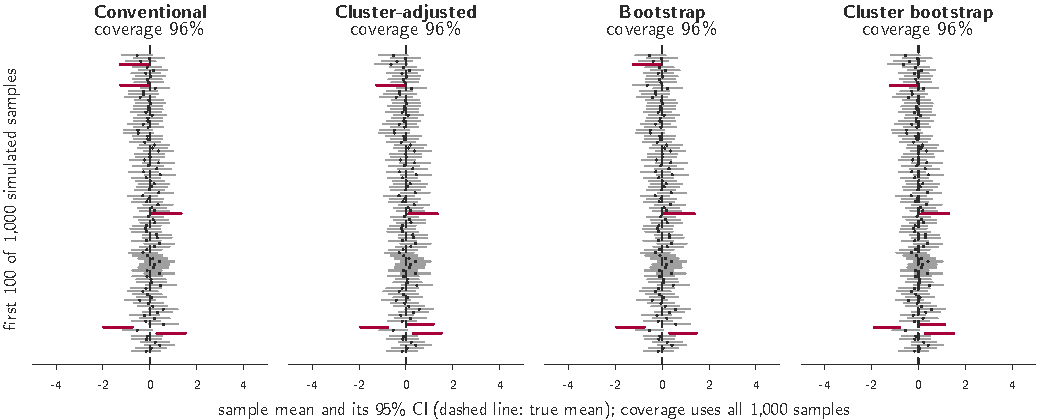
\includegraphics[height=0.70\textheight]{cluster_coverage_rho000.pdf}
\end{center}
}

\frame{
\frametitle{Relative Performance of Different Inference Procedures}
\small Given normally distributed clustered data, $\rho = 0.05$, $m=10$, $G=100$, $\alpha = 0.05$
\begin{center}
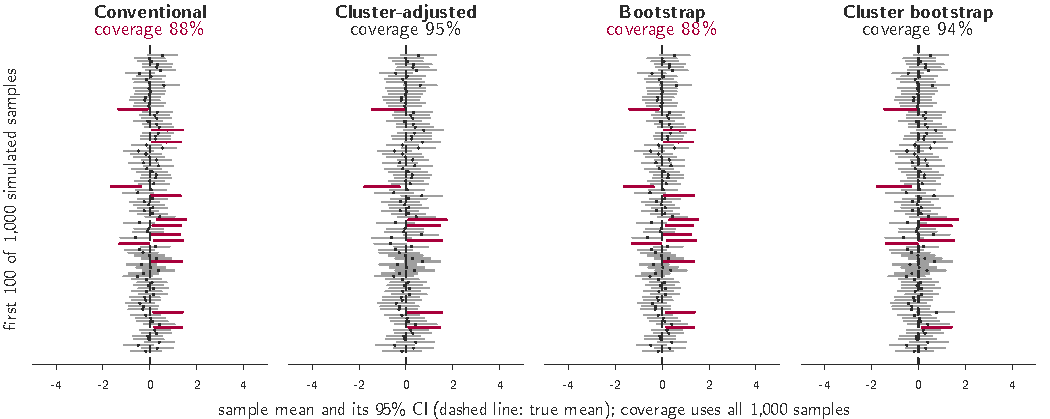
\includegraphics[height=0.70\textheight]{cluster_coverage_rho005.pdf}
\end{center}
}

\frame{
\frametitle{Relative Performance of Different Inference Procedures}
\small Given normally distributed clustered data, $\rho = 0.25$, $m=10$, $G=100$, $\alpha = 0.05$
\begin{center}
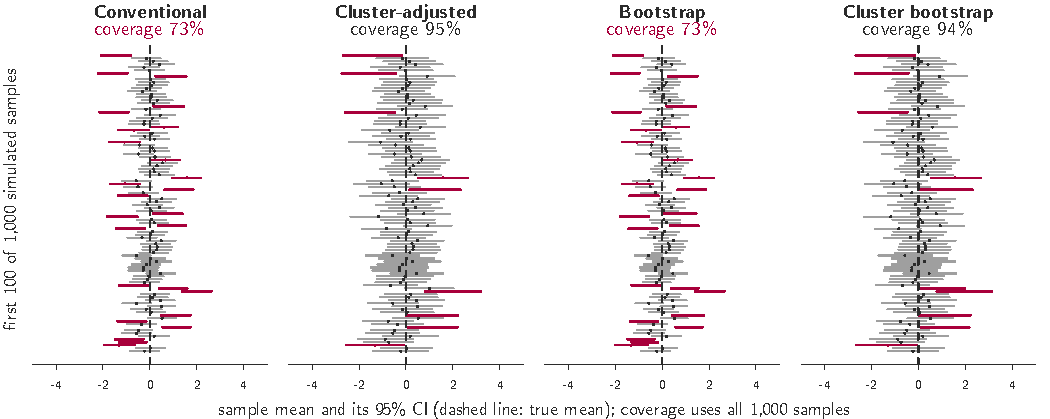
\includegraphics[height=0.70\textheight]{cluster_coverage_rho025.pdf}
\end{center}
}

\frame{
\frametitle{Relative Performance of Different Inference Procedures}
\small Given normally distributed clustered data, $\rho = 0.75$, $m=10$, $G=100$, $\alpha = 0.05$
\begin{center}
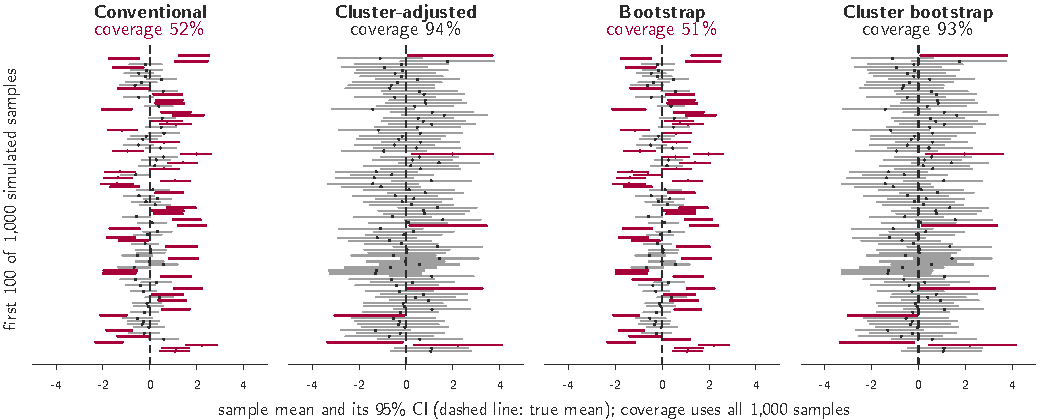
\includegraphics[height=0.70\textheight]{cluster_coverage_rho075.pdf}
\end{center}
}


\section{\texorpdfstring{Optional: Estimating $\Var(\bar{X})$ in Practice}{Optional: Estimating Var(X-bar) in Practice}}

\frame[label=estvar]{
\frametitle{(Optional) Estimating $\Var(\bar{X})$ in Practice}

%\textbf{Worksheet Q2}\bigskip

Under the same setup with equal cluster sizes, define the cluster means $\overline{X}_g=\frac{1}{m}\sum_{i=1}^m X_{gi}$ and the grand mean $\overline{X}=\frac{1}{G}\sum_{g=1}^G\overline{X}_g$. Let
\[
\text{MSW}=\frac{1}{G(m-1)}\sum_{g=1}^G\sum_{i=1}^m (X_{gi}-\overline{X}_g)^2,\qquad
\text{MSB}=\frac{m}{G-1}\sum_{g=1}^G(\overline{X}_g-\overline{X})^2.
\]

Standard (though rather complicated) ANOVA shows that $\E[\text{MSW}]=\sigma_W^2$ and $\E[\text{MSB}]=\sigma_W^2+m\sigma_B^2$.
}


\frame{
\frametitle{(Optional) Estimating $\Var(\bar{X})$ in Practice}
\textbf{Worksheet Q2}\bigskip

\begin{enumerate}
\item[(a)] Propose consistent estimators for $\sigma_W^2$, $\sigma_B^2$, and the intraclass correlation coefficient (ICC) $\rho=\sigma_B^2/(\sigma_B^2+\sigma_W^2)$.
\item[(b)] Using your results from (a), derive an estimator $\widehat{\Var}(\overline{X})$ for the sampling variance of the sample mean $\overline{X}$.
\item[(c)] Show that $\widehat{\rho}\xrightarrow{p}\rho$ and $\widehat{\Var}(\overline{X})/\Var(\overline{X})\xrightarrow{p}1$ as $G\to\infty$ with fixed $m$.
\item[(d)] Construct a $100(1-\alpha)\%$ cluster–adjusted confidence interval for $\mu$.
\end{enumerate}
}

% Restored 2026-09-17 at Yiqing's request (old slide 18); pset 3 will be updated instead.
\frame{
\frametitle{(Optional) Estimating $\Var(\bar{X})$ in Practice}

\begin{itemize}
\item Because $\{\overline{X}_g\}_{g=1}^G$ behave like $G$ approximately independent draws with variance $\sigma_B^2+\sigma_W^2/m$, small–sample inference for $\mu$ should use $(G-1)$ degrees of freedom. A cluster–adjusted CI is therefore
\[
\left[\overline{X}\ \pm\ t_{\alpha/2,(G-1)}\,\sqrt{\ \widehat{\Var}(\overline{X})\ }\right].
\]
\item Sanity checks:
\begin{itemize}
\item  If $\text{MSB}=\text{MSW}$ then $\widehat{\rho}=0$ and $\widehat{\Var}(\overline{X})=\widehat{\sigma}^2/n$ with $\widehat{\sigma}^2=\widehat{\sigma}_B^2+\widehat{\sigma}_W^2$ (the i.i.d. formula). 
\item If $\text{MSB}>\text{MSW}$, then $\widehat{\rho}>0$, the design effect $1+(m-1)\widehat{\rho}>1$, so this CI is (appropriately) wider than the conventional i.i.d. CI. 
\end{itemize}
\item In R, use the \texttt{anova()} function to obtain mean squares estimates. For better understanding, review ANOVA in greater depth.
\item Again, unbalanced cluster sizes make formulas messier. In practice, people often use the formulas above and set $m$ equal to the \emph{average sampled cluster size}. The more equal are the sampled cluster sizes, the more reasonable will be this simplification.
\end{itemize}
}


\section{Optional: Better Bootstrap Intervals}

\begin{frame}
\frametitle{(Optional) Percentile Interval: Recenter and Reverse}
The percentile CI treats the replications $\hat\theta_b^\ast$ as if they were draws of $\hat\theta$ around $\theta$.
The bootstrap analogy is about \emph{errors}: $\hat\theta^\ast-\hat\theta$ (resample vs.\ sample) mimics $\hat\theta-\theta$ (sample vs.\ population).
\begin{itemize}[<+->]
\item \alert{Recenter.} With $q^\ast_{.025}, q^\ast_{.975}$ the percentiles of the $\hat\theta_b^\ast$:
$$
\Pr\nolimits^\ast\big(q^\ast_{.025}-\hat\theta \le \hat\theta^\ast-\hat\theta \le q^\ast_{.975}-\hat\theta\big)=0.95
\ \ \Longrightarrow\ \
\Pr\big(q^\ast_{.025}-\hat\theta \le \hat\theta-\theta \le q^\ast_{.975}-\hat\theta\big)\approx 0.95
$$
\item \alert{Reverse.} Solve for $\theta$: \quad
$\big[\,2\hat\theta-q^\ast_{.975},\ \ 2\hat\theta-q^\ast_{.025}\,\big]$ \quad (the \alert{basic}, or reversed percentile, CI)
\begin{itemize}
\item A long right tail in the $\hat\theta_b^\ast$ becomes a long \emph{left} arm of the interval
\item Bias in the $\hat\theta_b^\ast$ is subtracted rather than added
\item If the $\hat\theta_b^\ast$ are symmetric around $\hat\theta$, the two intervals coincide
\end{itemize}
\item Median of the 20 incomes from Lecture 2-1 ($\hat\theta=65.25$): percentile CI $[43.5,\ 97.4]$; reversed CI $[33.1,\ 87.0]$
\item Which one is right depends on the statistic
\begin{itemize}
\item percentile CI: right if some monotone transformation $h$ makes $h(\hat\theta)-h(\theta)$ symmetric around 0, with the same distribution whatever $\theta$ is
\item reversed CI: right if $\hat\theta-\theta$ has the same distribution whatever $\theta$ is, e.g., a statistic with a stable bias
\end{itemize}
\end{itemize}
\end{frame}

\begin{frame}
\frametitle{(Optional) When Reversal Helps: A Biased Statistic}
The \alert{Gini coefficient} of 20 incomes drawn from the Lecture 2-1 population (true Gini 0.273)\par
\vspace{.3ex}
\parbox[t][2.6em][t]{\textwidth}{\small
\only<1|handout:0>{\emph{The truth}, which we can see only because we know the population: across samples of 20,
  the Gini averages 0.260. It is \alert{biased down} by 0.014.}%
\only<2|handout:0>{\emph{Our one sample}: $\widehat{\mathrm{Gini}}=0.308$. Its bootstrap replications average 0.295, or 0.013 below $\widehat{\mathrm{Gini}}$.
  The bootstrap \alert{copies the bias}.}%
\only<3|handout:0>{\emph{Percentile CI} $[0.220,\ 0.366]$ sits where the replications sit, below $\widehat{\mathrm{Gini}}$:
  it \alert{adds} the bias a second time.}%
\only<4|handout:1>{\emph{Reversed CI} $[0.250,\ 0.396]$: flipping each endpoint around $\widehat{\mathrm{Gini}}$ moves the interval up and
  \alert{removes} the bias.}%
\only<5|handout:2>{\emph{Coverage} over 4,000 samples per $n$: the reversed CI misses less, most of all in small samples.
  The gain is not universal: for the median ($n=20$), percentile 93\%, reversed 81\%; for a correlation of 0.8, percentile 92\%, reversed 85\%.}}
\vspace{-1ex}
\begin{center}
\only<1|handout:0>{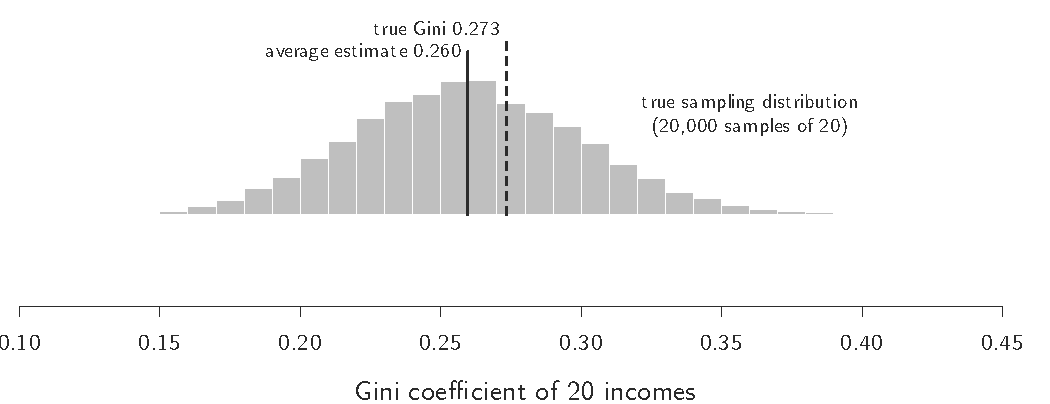
\includegraphics[height=0.59\textheight]{boot_gini_1.pdf}}%
\only<2|handout:0>{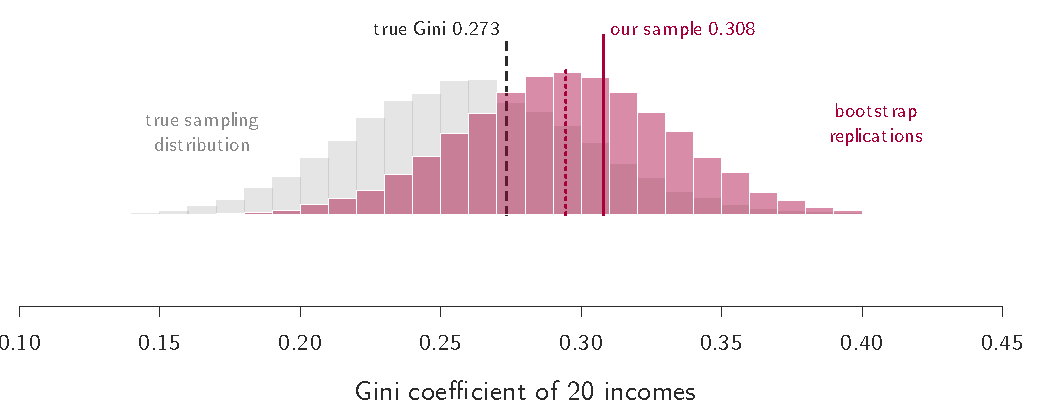
\includegraphics[height=0.59\textheight]{boot_gini_2.pdf}}%
\only<3|handout:0>{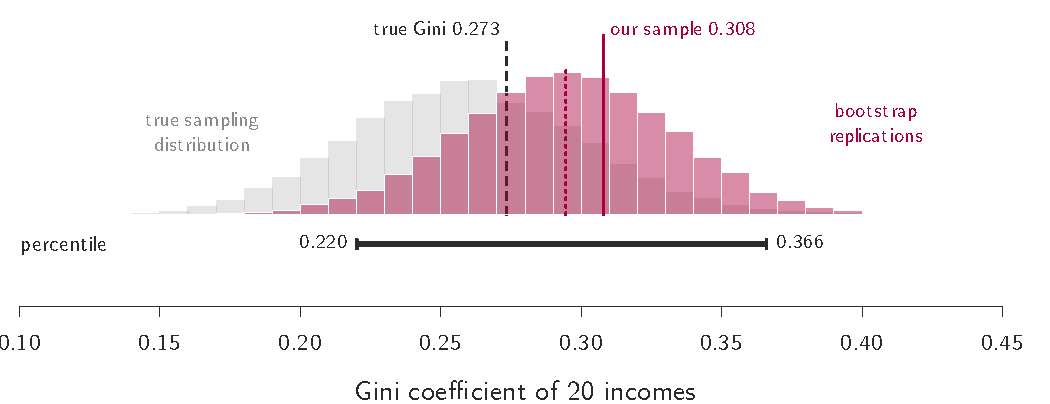
\includegraphics[height=0.59\textheight]{boot_gini_3.pdf}}%
\only<4|handout:1>{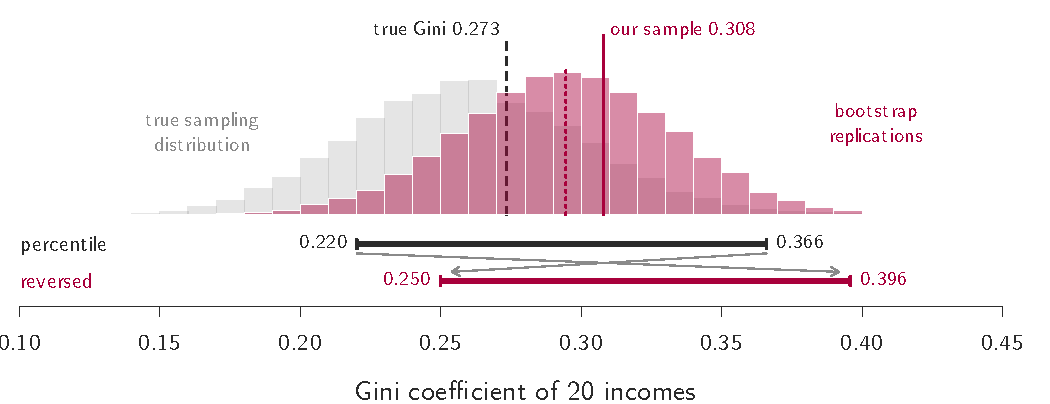
\includegraphics[height=0.59\textheight]{boot_gini_4.pdf}}%
\only<5|handout:2>{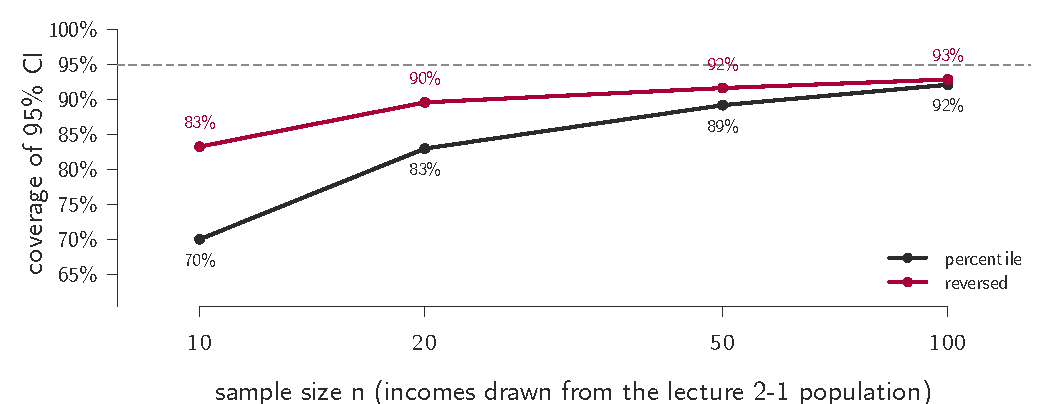
\includegraphics[height=0.59\textheight]{boot_gini_5.pdf}}
\end{center}
\end{frame}

\begin{frame}
\frametitle{(Optional) Refinement: Bootstrap-$t$}
The reversed CI assumes $\hat\theta-\theta$ has the same \emph{spread} in every sample. Often it does not: with right-skewed incomes, samples with a high mean also have a large $S$.
\begin{itemize}[<+->]
\item \alert{Studentize} each replication, using an SE computed inside resample $b$ (here $S_b^\ast/\sqrt{n}$):
$$
t_b^\ast=\frac{\hat\theta_b^\ast-\hat\theta}{\widehat{\rm se}_b^\ast}
\qquad\text{mimics}\qquad
\frac{\hat\theta-\theta}{\widehat{\rm se}}
$$
This ratio is approximately \alert{pivotal}: its distribution hardly depends on unknowns
\item Recenter and reverse as before, with the percentiles of the $t_b^\ast$ in place of the $t$-table:
\vspace{-.5ex}$$\big[\,\hat\theta-t^\ast_{.975}\,\widehat{\rm se},\ \ \hat\theta-t^\ast_{.025}\,\widehat{\rm se}\,\big]$$
\item Mean of the 20 incomes: $\hat\theta=72.76$, $\widehat{\rm se}=9.04$; $t^\ast_{.025}=-2.29$, $t^\ast_{.975}=1.98$ (the $t_{19}$ table: $\pm 2.09$)
\begin{itemize}
\item bootstrap-$t$ CI $[54.8,\ 93.4]$, longer on the right; \ $t$ CI $[53.8,\ 91.7]$; \ percentile $[55.7,\ 90.4]$
\end{itemize}
\item Why it helps: under regularity conditions, each tail's coverage error shrinks like $1/n$, not $1/\sqrt{n}$ as for the percentile and reversed CIs (Hall 1992)
\item Cost: an SE in every resample (for a median, a bootstrap inside each bootstrap). Alternative: BCa, \texttt{boot::boot.ci(type = "bca")}
\end{itemize}
\slidesource{Hall (1992), \emph{The Bootstrap and Edgeworth Expansion}, Springer, Ch.~3}
\end{frame}

\begin{frame}
\frametitle{(Optional) When Bootstrap-$t$ Helps: Skewed Data}
The mean of right-skewed incomes: samples of 20 from the Lecture 2-1 population (true mean 72.0)\par
\vspace{.3ex}
\parbox[t][2.6em][t]{\textwidth}{\small
\only<1|handout:0>{1,000 of 50,000 samples: a high mean comes with a large $S$ (correlation 0.54 over all 50,000). Low-mean samples get
  \alert{short} intervals, so the $t$ interval misses below the truth far more often than above (40 vs.\ 8).}%
\only<2|handout:0>{So the true $t$-ratio is \alert{skewed}: its 2.5\% and 97.5\% points are $-2.51$ and $1.81$, not $\pm 2.09$.}%
\only<3|handout:1>{The bootstrap $t^\ast$ from our one sample \alert{catches much of the skew}: $-2.29$ and $1.98$.}%
\only<4|handout:2>{\emph{Coverage} over 10,000 samples per $n$. At $n=20$: bootstrap-$t$ 94.7\%, $t$ 94.1\%, percentile 91.8\%, reversed 91.3\%.
  Bootstrap-$t$ also \alert{balances the misses}: 3.2\% below and 2.1\% above, against 4.7\% and 1.3\% for $t$.}}
\vspace{-1ex}
\begin{center}
\only<1|handout:0>{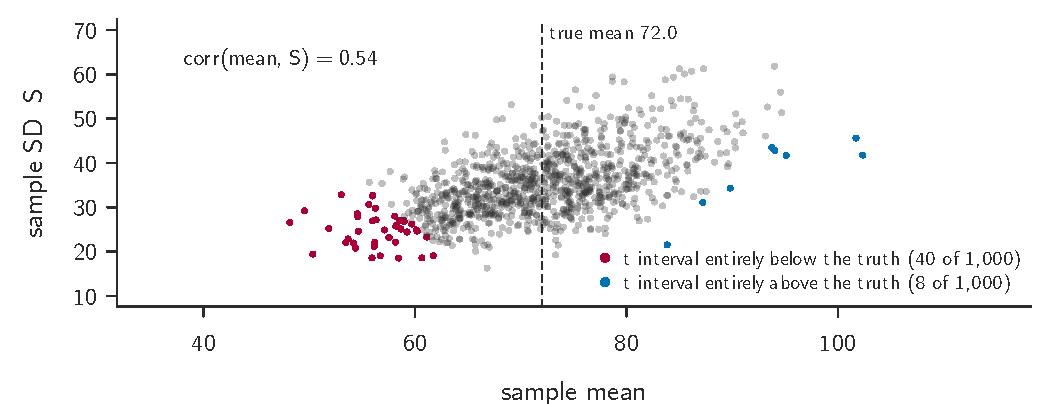
\includegraphics[height=0.59\textheight]{boot_t_1.pdf}}%
\only<2|handout:0>{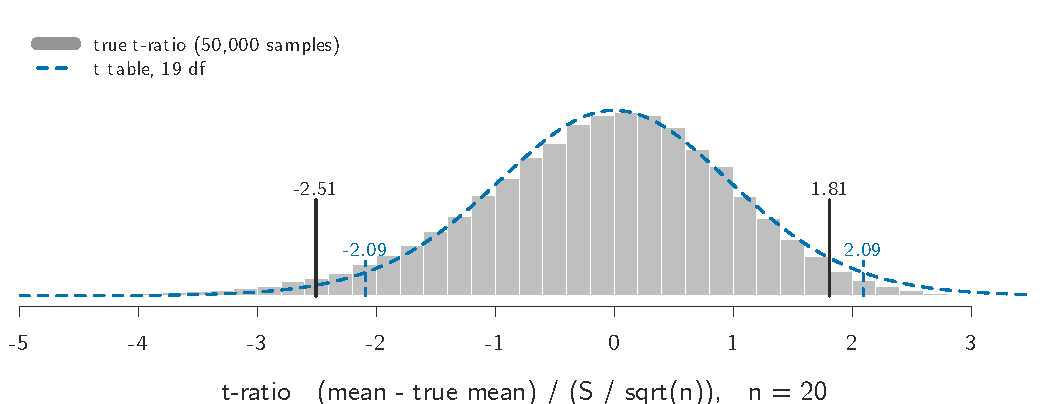
\includegraphics[height=0.59\textheight]{boot_t_2.pdf}}%
\only<3|handout:1>{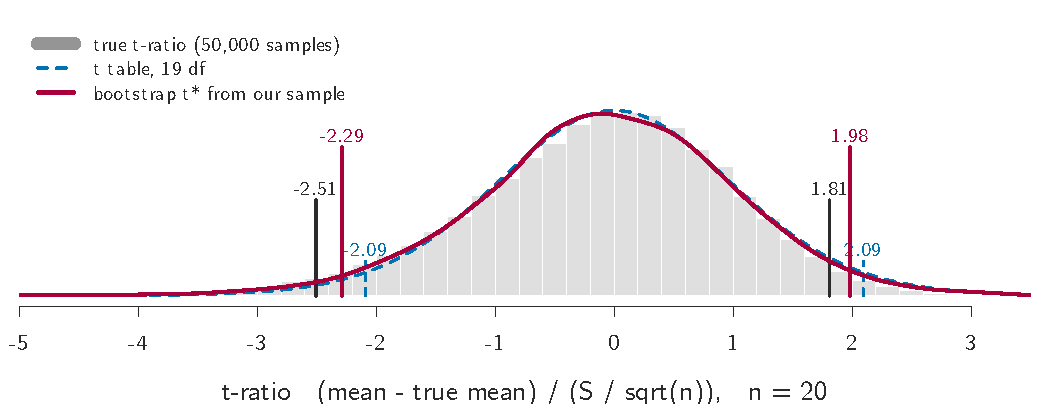
\includegraphics[height=0.59\textheight]{boot_t_3.pdf}}%
\only<4|handout:2>{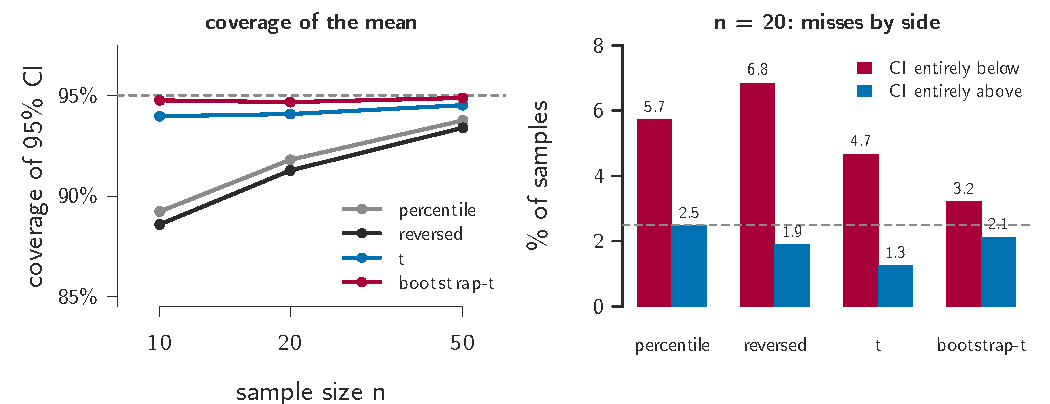
\includegraphics[height=0.59\textheight]{boot_t_4.pdf}}
\end{center}
\end{frame}

\end{document}
